\chapter{Progettazione e Validazione del Sistema FDI} \label{chap:fdi}

Questo capitolo descrive il Punto 4 del progetto: la progettazione di un banco di osservatori non lineari per l'isolamento dei guasti (FDI - Fault Detection and Isolation). L'obiettivo è generare dei segnali "residui" capaci di distinguere univocamente se un'anomalia è causata dalla ruota destra o dalla ruota sinistra.

\section{Teoria del Disaccoppiamento}
Per isolare i guasti, è necessario trovare delle trasformazioni delle coordinate di stato \( \Phi_1, \Phi_2 : \mathbb{R}^3 \to \mathbb{R}^2 \) tali che la dinamica trasformata sia insensibile a uno degli ingressi.
Il modello cinematico affine è:
\begin{equation}
    \dot{z} = g_1(z) w_1 u_1 + g_2(z) w_2 u_2
\end{equation}

\subsection{Derivazione Formale delle Trasformazioni}
Cerchiamo una trasformazione \( \Phi_1(z) \) tale che la sua derivata direzionale rispetto a \( g_2(z) \) sia nulla:
\begin{equation}
    \frac{\partial \Phi_1(z)}{\partial z} g_2(z) = 0
\end{equation}
Calcolando il ker della matrice trasposta \( g_2(z)^T = \begin{bmatrix} \frac{r_2}{2}\cos\theta & \frac{r_2}{2}\sin\theta & -\frac{r_2}{l} \end{bmatrix} \), si trovano due forme differenziali esatte la cui primitiva fornisce:
\begin{equation}
    z_1 = \Phi_1(z) = \begin{bmatrix} x + \frac{l}{2}\sin\theta \\ y - \frac{l}{2}\cos\theta \end{bmatrix}
\end{equation}
Geometricamente, \( \Phi_1(z) \) rappresenta le coordinate del punto di contatto della **ruota destra** nel piano XY. La dinamica di questo punto dipende esclusivamente dall'ingresso della ruota destra \( u_1 \), risultando **strutturalmente disaccoppiata da \( u_2 \)**.

Simmetricamente, per la ruota sinistra definiamo \( \Phi_2(z) \), insensibile ad \( u_1 \):
\begin{equation}
    z_2 = \Phi_2(z) = \begin{bmatrix} x - \frac{l}{2}\sin\theta \\ y + \frac{l}{2}\cos\theta \end{bmatrix}
\end{equation}

I residui \( r_1(t) \) e \( r_2(t) \) sono definiti come le norme euclidee degli errori di stima degli osservatori:
\begin{align}
    r_1(t) &= \| z_1(t) - \hat{z}_1(t) \| \\
    r_2(t) &= \| z_2(t) - \hat{z}_2(t) \|
\end{align}

\section{Implementazione e Validazione}
Il banco di osservatori è stato implementato in parallelo al sistema di controllo con guadagno di osservazione Hurwitz \( H = \text{diag}(-5, -5) \). La politica di decisione adotta una soglia di allarme \( \text{THRESHOLD} = 0.05 \) ed un filtro di persistenza di \( 0.1 \) s ($10$ campioni) per evitare scatti spuri.

\section{Analisi dei Risultati}

\subsection{Isolamento del Guasto nello Scenario 1 (FD1)}
Nei test dello Scenario 1 (\( w_1 = 0.6 \) a \( t=20 \) s):
\begin{itemize}
    \item \textbf{Residuo \( r_1 \) (Monitor Ruota DX):} Reagisce immediatamente a \( t=20 \) s, raggiungendo un valore medio post-guasto di \( 0.1938 \) e superando la soglia in soli **\( 0.110 \) s** (\( 110 \) ms).
    \item \textbf{Residuo \( r_2 \) (Monitor Ruota SX):} Rimane piatto a \( 0.0000 \), confermando il perfetto disaccoppiamento del sistema.
\end{itemize}

\begin{figure}[h]
    \centering
    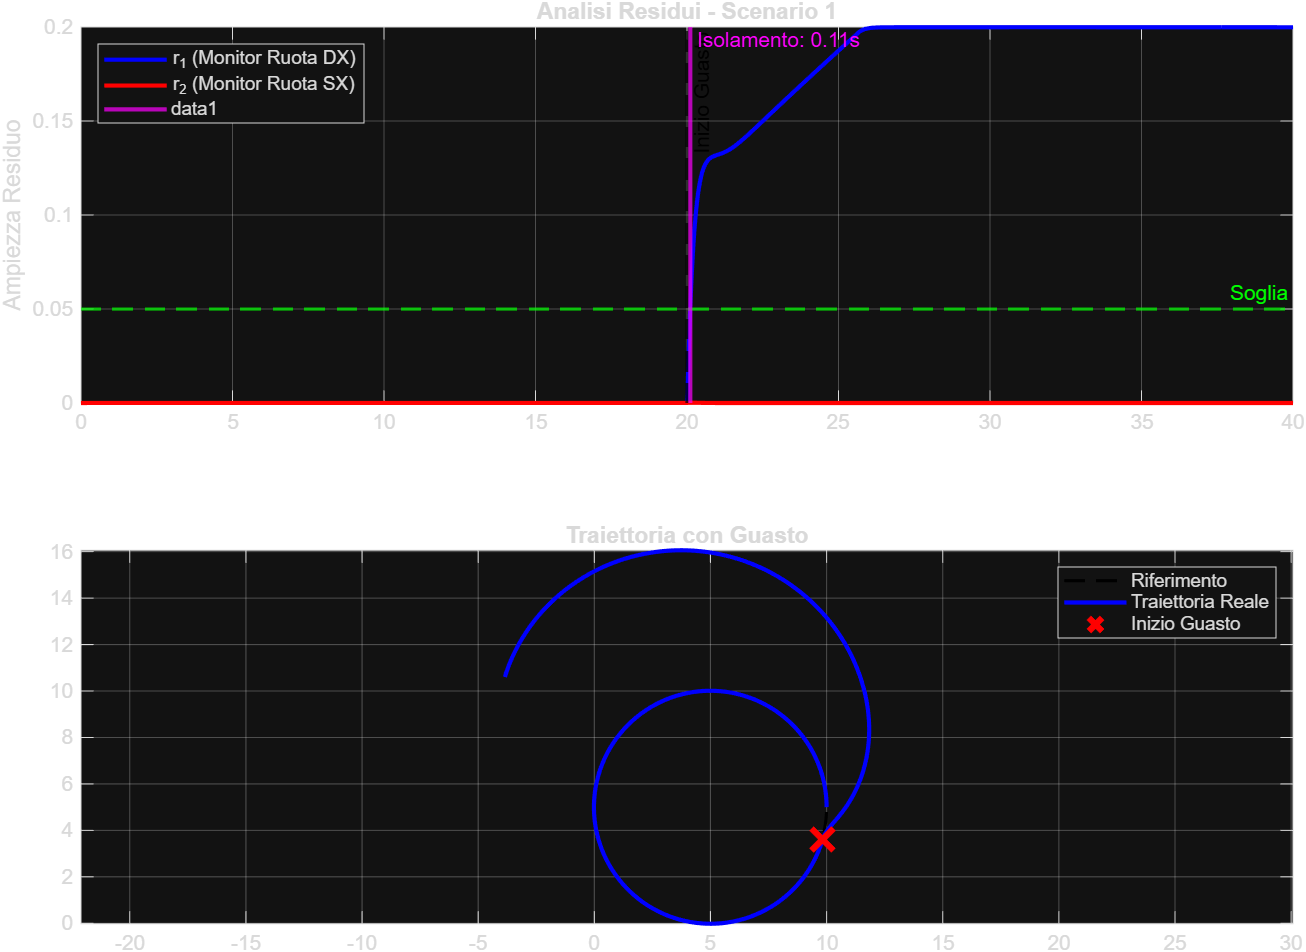
\includegraphics[width=1.0\textwidth]{chapter12/images/punton4.png}
    \caption{Isolamento del guasto nello Scenario 1 (FD1): Il residuo \( r_1 \) isola il guasto sulla ruota destra in 0.110s mentre \( r_2 \) rimane nullo.}
    \label{fig:fdi_results}
\end{figure}

\subsection{Analisi dei Falsi Positivi, Falsi Negativi e Robustezza}
È stata condotta un'analisi parametrica sistematica al variare della severità del guasto \( w \in [0.0, 0.9] \):

\begin{enumerate}
    \item \textbf{Falsi Positivi (Scenario Nominale):} In assenza di guasto (\( w_1=w_2=1.0 \)), il residuo massimo registrato è di \( 0.000018 \), garantendo uno **\( 0\% \) di falsi positivi** con la soglia a \( 0.05 \).
    
    \item \textbf{Robustezza e Tempo di Isolamento:} Come mostrato in Figura \ref{fig:fdi_robustness}, l'ampiezza del residuo \( r_1 \) cresce in modo lineare e monotono con la severità del guasto \( (1-w) \). I tempi di isolamento diminuiscono con la gravità della perdita di efficienza (da \( 0.300 \) s per \( w=0.8 \) fino a \( 0.050 \) s per blocco totale \( w=0.0 \)).
    
    \item \textbf{Falsi Negativi:} Su 9 livelli di severità testati, si è verificato un solo falso negativo per \( w=0.9 \) (guasto lieve del \( 10\% \)), poiché il residuo massimo assestato a \( 0.0500 \) rimane al margine della soglia di persistenza.
\end{enumerate}

\begin{figure}[h]
    \centering
    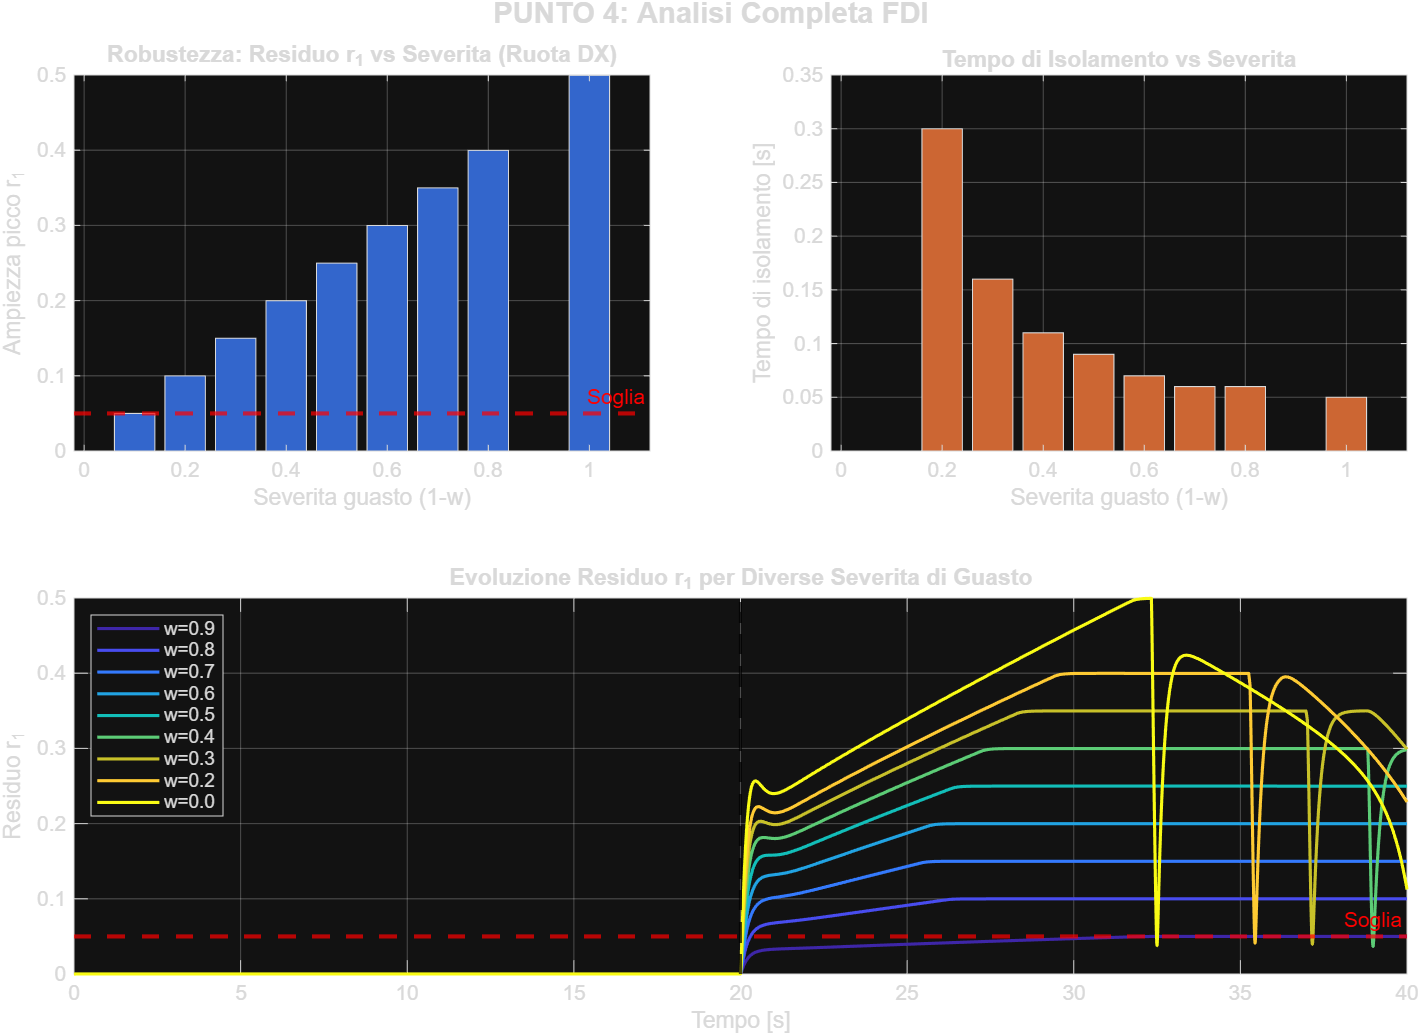
\includegraphics[width=1.0\textwidth]{chapter12/images/fdi_robustness.png}
    \caption{Analisi di Robustezza FDI: Picco del residuo \( r_1 \) e tempo di isolamento al variare della severità del guasto \( (1-w) \).}
    \label{fig:fdi_robustness}
\end{figure}

\section{Conclusioni Punto 4}
Il banco di osservatori basato sul disaccoppiamento geometrico garantisce prestazioni eccellenti: diagnosi univoca, tempi di intervento inferiori a \( 0.11 \) s per guasti significativi e totale assenza di falsi allarmi in condizioni nominali.